\section{Experimental Results}

\begin{figure}[h]
    \centering
    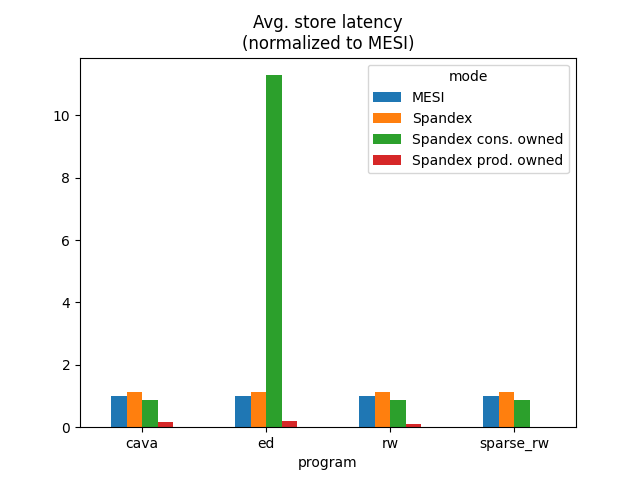
\includegraphics[width=0.45\textwidth]{stores.png}
    \caption{Average Store Latency}
    \label{fig:stores}
\end{figure}

\begin{figure}[h]
    \centering
    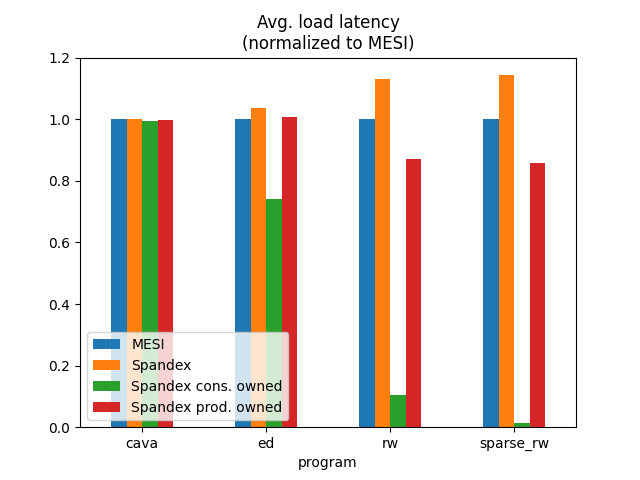
\includegraphics[width=0.45\textwidth]{loads.png}
    \caption{Average Load Latency}
    \label{fig:loads}
\end{figure}

\begin{figure}[h]
    \centering
    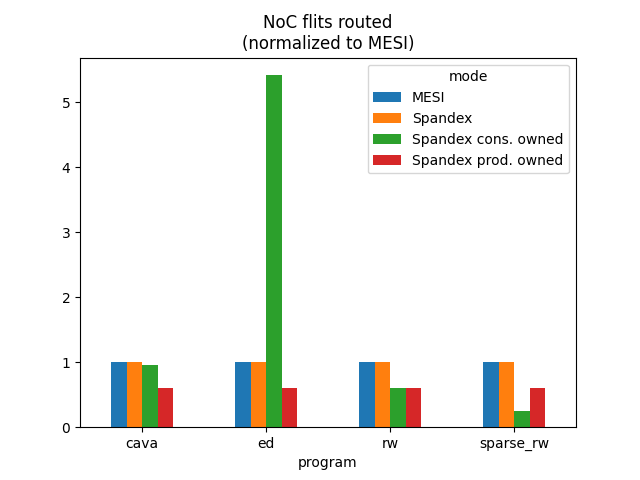
\includegraphics[width=0.45\textwidth]{traffic.png}
    \caption{NoC Traffic Routed}
    \label{fig:traffic}
\end{figure}

Average store latency is least with Spandex producer-owned lines while load latency is least with Spandex consumer-owned lines, both as expected. However, the magnitude of the effect varies widely with the application, by what we believe to be the sparsity of loads relative to the sparsity of stores. NoC usage is least for better for Spandex consumer-owned when the accesses are sparse, and Spandex producer-owned when they are dense.

We believe \verb+ed+ suffers high NoC traffic with Spandex consumer-owned (\(\sim\)10x MESI case) because it has several for-loops that cut `against the grain', so the stores are unable to be coalesced. However, MESI can still exploit reuse, because it brings the whole line to the writer, so future writes to that line hit \textit{for the duration of the epoch, instead of for the duration of the coalescing window}.

Currently, our compiler pass would select the same kind of request-type mapping for all producer/consumer relationships, so we would select a good all-around cache optimization, like producer-owned for these accesses. This is still dynamic in the sense that accesses outside of the producer/consumer relationship will be regular Spandex requests, while producer/consumer accesses are optimized. However, future work could look at the sparsity of loads and stores and decide for each producer/consumer pair which cache optimization to apply. The benchmarks we ran indicate that when trying to optimize NoC traffic, some cases  (\verb+cava+, \verb+ed+, and \verb+rw+) would want producer-owned, but others (\verb+sparse_rw+) would want consumer-owned. NoC traffic routed correlates well with energy utilization, as much of the energy is spent in the interconnect, so this optimization is important for low-power devices \cite{low_energy_FPGA}. Optimizing for runtime, however, is somewhat more nuanced due to parallelism.

We do not know exactly how the load-latency and store-latency effects the runtime of each benchmark, and we could not simulate the benchmarks for the reasons outlined in \cref{sec:methods}. The effect of store-latency is partially isolated by the MSHR buffer. It is probable that \verb+ed+ has such a large average store latency that it would fill the MSHR and induce stalls. The impact of load-latency on runtime is also not straightforward because the processor may be able to execute independent instructions out-of-order while waiting for a load. However, many important programs are memory-bound, so these would be sensitive to the load-latency. For example, linked-list traversals would be strongly affected by load-latency.